\documentclass[12pt]{report}

\usepackage{amsmath}
\usepackage{pgfplots}
\usepgfplotslibrary{units}
\usepackage[russian]{babel}
\usepackage{filecontents}
\usepackage{titlesec, blindtext, color}
\usepackage{listings}

\usepackage{titlesec, blindtext, color} 
\definecolor{gray75}{gray}{0.75} 
\newcommand{\hsp}{\hspace{20pt}} 

\usepackage{geometry}
\geometry{top=0.5cm}


\lstset{ 
language=haskell,                 
basicstyle=\small\sffamily, 
numbers=left,              
numberstyle=\tiny,        
stepnumber=1,              
numbersep=5pt,             
showspaces=false,          
showstringspaces=false,   
showtabs=false,             
frame=single,            
tabsize=2,                
captionpos=t,              
breaklines=true,           
breakatwhitespace=false, 
escapeinside={\#*}{*)}   
}

\titleformat{\chapter}[hang]{\Huge\bfseries}{\thechapter\hsp\textcolor{gray75}{|}\hsp}{0pt}{\Huge\bfseries}

\begin{filecontents}{uMult.dat}
1000 0.0059538099999999995
1100 0.00650186
1200 0.00500285
1300 0.00555337
1400 0.008996299999999999
1500 0.00995671
1600 0.009855840000000001
1700 0.019011860000000002
1800 0.01801024
1900 0.0252644
2000 0.01061246
\end{filecontents}

\begin{filecontents}{uMultLib.dat}
1000 0.28866500000000006
1100 0.33328877000000007
1200 0.4018312
1300 0.41553629000000003
1400 0.51159321
1500 0.5524156800000001
1600 0.8165667799999999
1700 0.90921932
1800 0.97125617
1900 1.0638098200000001
2000 1.1544614
\end{filecontents}

\begin{filecontents}{wMult.dat}
1000 0.16954728000000002
1100 0.19832370000000002
1200 0.23013233
1300 0.28036073
1400 0.31670195
1500 0.35118906
1600 0.39693935
1700 0.44291941
1800 0.4905573200000001
1900 0.54654837
2000 0.6031616900000001
\end{filecontents}

\begin{filecontents}{wMultU1.dat}
1000 0.12036883000000001
1100 0.14067822000000002
1200 0.18502324000000003
1300 0.24424469
1400 0.26929561
1500 0.30338711999999995
1600 0.33407759000000004
1700 0.37459303000000005
1800 0.41933486000000003
1900 0.44667912000000004
2000 0.4900813200000001
\end{filecontents}

\begin{filecontents}{wMultU2.dat}
1000 0.13563091
1100 0.18681058
1200 0.20674228
1300 0.21943319
1400 0.24889928
1500 0.28773166
1600 0.31988548
1700 0.36126201
1800 0.47617364999999995
1900 0.52927952
2000 0.5833035200000001
\end{filecontents}

\begin{filecontents}{wMultU3.dat}
1000 0.01285779
1100 0.011855799999999998
1200 0.01610728
1300 0.02106222
1400 0.026515760000000006
1500 0.01720994
1600 0.028615970000000008
1700 0.03922262000000001
1800 0.04632705
1900 0.04538006
2000 0.03576978
\end{filecontents}

\begin{document}

\begin{titlepage}
	\centering
	{\scshape\LARGE МГТУ им. Баумана \par}
	\vspace{3cm}
	{\scshape\Large Лабораторная работа №2\par}
	\vspace{0.5cm}	
	{\scshape\Large По курсу: "Анализ алгоритмов"\par}
	\vspace{1.5cm}
	{\huge\bfseries Умножение матриц\par}
	\vspace{2cm}
	\Large Работу выполнила: Подвашецкий Дмитрий, ИУ7-54Б\par
	\vspace{0.5cm}
	\LargeПреподаватели:  Волкова Л.Л., Строганов Ю.В.\par

	\vfill
	\large \textit {Москва, 2019} \par
\end{titlepage}

\tableofcontents

\newpage
\chapter*{Введение}
\addcontentsline{toc}{chapter}{Введение}

\textbf{Матрица} - математический объект, записываемый в виде прямоугольной таблицы элементов кольца или поля которая представляет собой совокупность строк и столбцов, на пересечении которых находятся её элементы.

Матрицы широко применяются в математике для компактной записи систем линейных алгебраических или дифференциальных уравнений. В этом случае, количество строк матрицы соответствует числу уравнений, а количество столбцов — количеству неизвестных. В результате решение систем линейных уравнений сводится к операциям над матрицами.

Матрицы допускают следующие алгебраические операции:
\begin{enumerate}
	\item сложение матриц, имеющих один и тот же размер;
	\item умножение матриц подходящего размера;
	\item умножение матрицы на элемент основного кольца или поля;
\end{enumerate}

\textbf{Умножение матриц} - одна из основных операций над матрицами.

Целью данной лабораторной работы является реализация и изучение алгоритма умножения матриц методом Винограда и стандартного.

\textbf{Задачами} данной лабораторной являются:
\begin{enumerate}
	\item изучение стандарного метода и метода Винограда для умножения матриц;
	\item реализация данных двух методов, а так же оптимизация последнего;
	\item теоретический анализ трудоемкости рассматриваемых алгоритмов;
	\item экспериментальное подтверждение различий во временнóй эффективности рассматриваемых алгоритмов;
	\item описание и обоснование полученных результатов в отчете о выполненной лабораторной
работе, выполненного как расчётно-пояснительная записка к работе.
\end{enumerate}

\chapter{Аналитическая часть}
Операция умножения матриц повсеместно приминяется в математике, физике, программировании и т.д.
Для того, чтобы произведение матрицы A, размерами n на m, на матрицу B, размерами u на v, было возможно, необходимо, чтобы n = u.

В данной лабораторной работе я рассмотрю два алгоритма умножения матриц.

Первый алгоритм - стандартный. 

Пусть есть две матрицы: 
\begin{center}
{$
A_{nm} = 
\begin{pmatrix}
  a_{00} &  ... & a_{0m}\\
   ... & ... & ...\\
  a_{n0} &  ... &  a_{nm}
\end{pmatrix}
$};
{$
B_{mk} = 
\begin{pmatrix}
  b_{00} &  ... & b_{0k}\\
   ... & ... & ...\\
  b_{m0} &  ... &  b_{mk}
\end{pmatrix}
$}
\end{center}

Тогда, пусть:
\begin{center}
{$
C_{nk} = A_{nm}B_{mk}
$} 
\end{center}
Где ij эллемент матрицы {$C_{nk}$} вычисляется как скалярное произведение i строки матрицы  {$A_{nm}$} на j столбец матрицы {$B_{mk}$}.

\begin{equation}
C_{ij} = a_{0i} * b_{j0} + ... + a_{mi} * b_{jm},  i = [1..n], j = [1..m]
\end{equation}

Второй алгоритм - Винограда.

В данном алгоритме, также как и в предыдущем, каждый элемент производной матрицы считается как скалярное произведение.
Рассмотрим два вектора:
\begin{center}
{$
V = 
\begin{pmatrix}
  v1 & v2 & v3 & v4
\end{pmatrix}
$}

{$
W = 
\begin{pmatrix}
  w1 & w2 & w3 & w4
\end{pmatrix}
$}
\end{center}

Их скалярное произведение равно:
\begin{equation}
V*W = v1w1 + v2w2 + v3w3 + v4w4
\end{equation}

Выражение (1.2) можно переписать:
\begin{equation}
V*W = (v1 + w2)(v2 + w1) + (v3 + v4)(v4 + w3) - v1v2 - v3v4 - w1w2 - w3w4
\end{equation}

Можно заметить, что правую часть данного выражения можно высчитать заранее для каждого вектора.
Это означает, что, при предварительной обработке векторов мы можем, в дальнейшем, сэкономить 2 операции умножения, за счет 2х лишних операций сложения.

Если при умножении двух матриц произвести обработку строк первой и столбцов второй, то можно добиться большей эффективности по времени. [1]

\chapter{Конструкторская часть}
\section{Схемы алгоритмов}

\begin{center}
    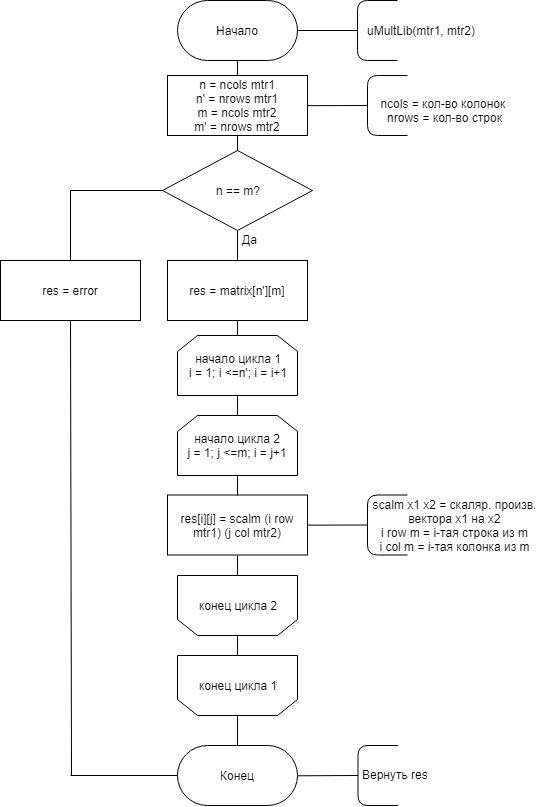
\includegraphics[scale=0.6]{UsualMult}

    Схема 1. Стандартный алгоритм умножения

    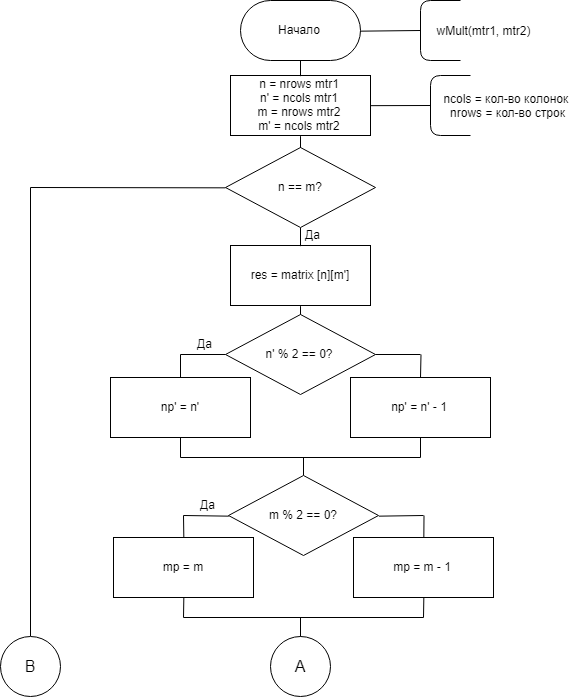
\includegraphics[scale=0.7]{WinogradMult}

	 Схема 2.1. Aлгоритм умножения методом Винограда

    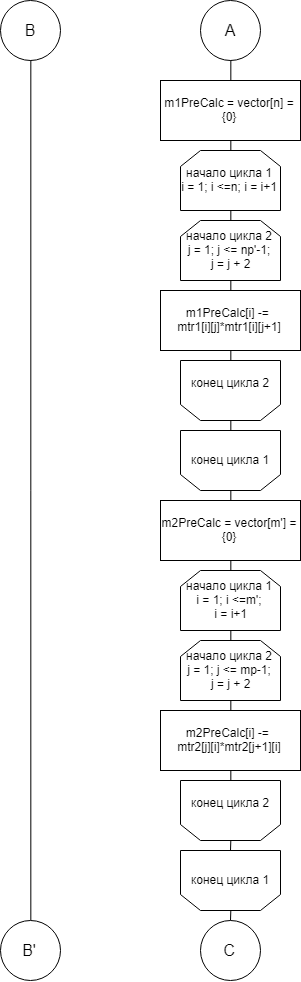
\includegraphics[scale=0.65]{WinogradMult2}

	 Схема 2.2. Aлгоритм умножения методом Винограда

    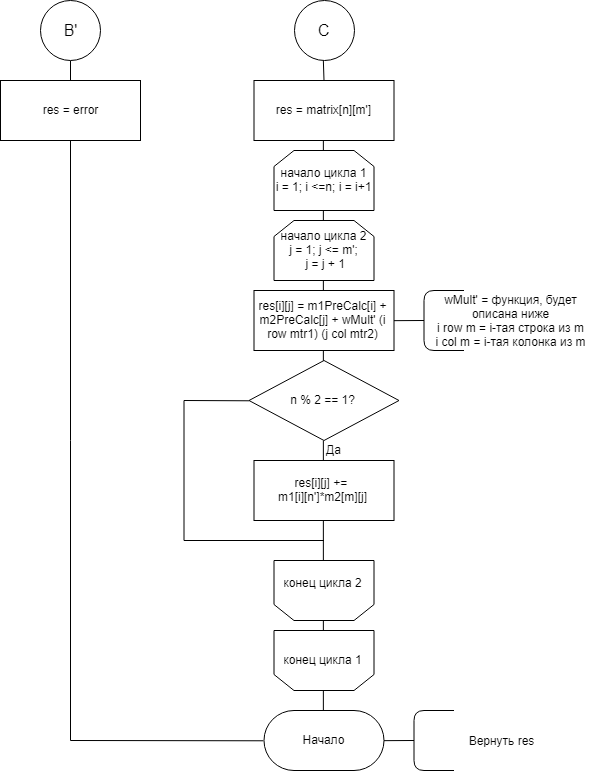
\includegraphics[scale=0.7]{WinogradMult3}

    Схема 2.3. Aлгоритм умножения методом Винограда

    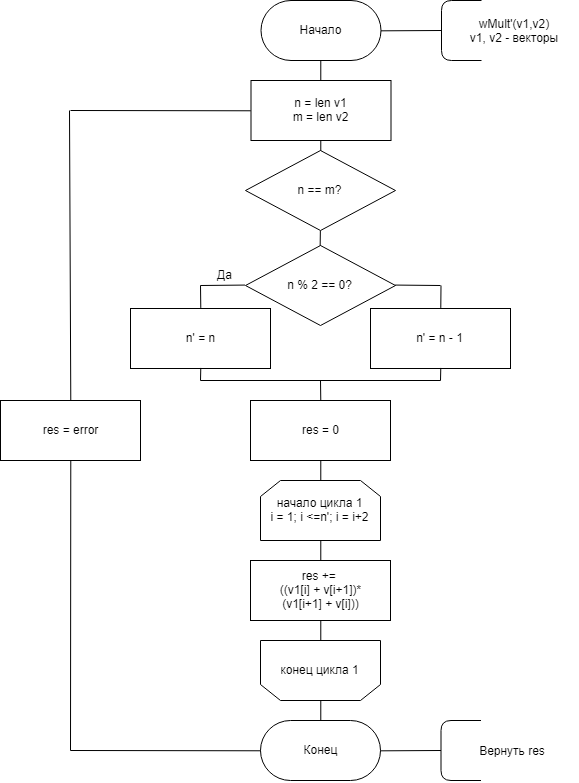
\includegraphics[scale=0.7]{wMult}

    Схема 3. Функция wMult' (для Схема. 2.3.)
\end{center}

\chapter{Технологическая часть}
\section{Выбор ЯП}
В качестве языка программирования был выбран Haskell, для ознакомления с ним.

\section{Замеры времени}
Замер времени работы алгоритмов производился при помощи функций getCurrentTime, diffUTCTime из библиотеки Data.Time.Clock. [2]

Также производится усреднение времени работы улгоритмов. Для этого время считается для 10 вызовов, и после делится на 10.

\section{Работа с матрицами}
Для обработки матриц использовалась библиотека Data.Matrix, на ряду с массивом массивов. [3]

\section{Требования к ПО}

\textbf{Требования к вводу:}
\begin{enumerate}
	\item Имя файла, содержащего значения первой матрицы
	\item Имя файла, содержащего значения второй матрицы
\end{enumerate}
\textbf{Требования к программе:}
\begin{enumerate}
  	\item Корректный ввод, корректный вывод, программа не должна аварийно завершаться
\end{enumerate}

\textbf{Требования структуре входного файла:}
	Значения в строках должны быть записаны на одной строке. Разделитель - пробел. Конец строки - переход на новую строку.
	
	Пример:
\begin{center}
	1 2

	3 4
\end{center}

\section{Сведения о модулях программы}
Программа состоит из:
\begin{itemize}
	\item main.hs - главный файл программы
	\item UsualMultLib.hs - файл с функцией вычисления произведения матриц стандартным алгоритмом (Листинг 3.1.)
	\item WinogradMult.hs - файл с функцией вычисления произведения матриц методом Винограда (Листинг 3.2.)
	\item WinogradMultU1.hs - файл с первой модификацией метода Винограда (Листинг 3.3.)
	\item WinogradMultU2.hs - файл со второй модификацией метода Винограда (Листинг 3.4.)
	\item WinogradMultU3.hs - файл с третьей модификацией метода Винограда (Листинг 3.5.)
\end{itemize}

\begin{lstlisting}[label=some-code,caption=Стандартный алгоритм]
scalm' :: (Num a) => Vector a -> Vector a -> a
scalm' v1 v2 = 
        if V.length v1 == V.length v2
            then Prelude.sum( [(unsafeIndex v1 i)*(unsafeIndex v2 i) | i <- [0..(V.length v1)-1]] )
            else error "Mtr.size.Error"

uMultLib :: (Num a) => Matrix a -> Matrix a -> Matrix a
uMultLib m1 m2 = do
    if n' == m
        then fromLists [[scalm' (getRow i m1) (getCol j m2) | j <- [1..m]] | i <- [1..n']]
        else error "Mtr.size.Error"
            where 
                n = ncols m1
                m = nrows m2

                n' = nrows m1
                m' = ncols m2
\end{lstlisting}

\begin{lstlisting}[label=some-code,caption=Алгоритм Винограда]
wMult :: (Num a) => Matrix a -> Matrix a -> Matrix a
wMult m1 m2 = 
    if m == n'
        then res 
        else error "Mtr.Size.Error"
    where
        n = nrows m1
        n' = ncols m1
        m = nrows m2
        m' = ncols m2

        np' = if even n' then n' else n' - 1
        mp = if even m then m else m - 1

        m1PreCalc = [Prelude.sum ([-1*(getElem i j m1)*(getElem i (j+1) m1) | j <- [1, 3..np'-1]]) | i <- [1..n]]  
        m2PreCalc = [Prelude.sum ([-1*(getElem j i m2)*(getElem (j+1) i m2) | j <- [1, 3..mp-1]]) | i <- [1..m']]

        res = matrix n m' $ \(i,j) ->
                (m1PreCalc !! (i-1)) + (m2PreCalc !! (j-1)) +  
                wMult' (getRow i m1) (getCol j m2) + 
                if odd n' then getElem i n' m1 * getElem m j m2 else 0

wMult' :: (Num a) => Vector a -> Vector a -> a
wMult' v1 v2 = 
    if n == m
        then res
        else error "Oh no, smth goes wrong"
    where
        n = Data.Vector.length v1
        m = Data.Vector.length v2

        n' = if even n then n else n-1

        res = Prelude.sum ( [ ((unsafeIndex v1 i) + (unsafeIndex v2 (i+1)))*
                              ((unsafeIndex v1 (i+1) + (unsafeIndex v2 i))) | i <- [0, 2..n'-2] ] )
\end{lstlisting}

\begin{lstlisting}[label=some-code,caption=Алгоритм Винограда модификация 1]
wMultU1 :: (Num a) => Matrix a -> Matrix a -> Matrix a
wMultU1 m1 m2 = 
    if m == n'
        then res 
        else error "Mtr.Size.Error"
    where
        n = nrows m1
        n' = ncols m1
        m = nrows m2
        m' = ncols m2

        np' = if even n' then n' else n' - 1
        mp = if even m then m else m - 1

        m1PreCalc = [Prelude.sum ([-1*(getElem i j m1)*(getElem i (j+1) m1) | j <- [1, 3..np'-1]])
                         | i <- [1..n]]
        m2PreCalc = [Prelude.sum ([-1*(getElem j i m2)*(getElem (j+1) i m2) | j <- [1, 3..mp-1]])
                         | i <- [1..m']]

        res = matrix n m' $ \(i,j) ->
                (m1PreCalc !! (i-1)) + (m2PreCalc !! (j-1)) +  
                wMultU1' (getRow i m1) n (getCol j m2) m' + 
                if odd n' then getElem i n' m1 * getElem m j m2 else 0

wMultU1' :: (Num a) => Vector a -> Int -> Vector a -> Int -> a
wMultU1' v1 n v2 m = 
    if n == m
        then res
        else error "Oh no, smth goes wrong"
    where
        n' = if even n then n else n-1

        res = Prelude.sum ( [ ((unsafeIndex v1 i) + (unsafeIndex v2 (i+1)))*
                              ((unsafeIndex v1 (i+1) + (unsafeIndex v2 i))) | i <- [0, 2..n'-2] ] )
\end{lstlisting}

\begin{lstlisting}[label=some-code,caption=Алгоритм Винограда модификация 2]
wMultU2 :: (Num a) => Matrix a -> Matrix a -> Matrix a
wMultU2 m1 m2 = 
    if m == n'
        then res
        else error "Mtr.Size.Error"
    where
        n = nrows m1
        n' = ncols m1
        m = nrows m2
        m' = ncols m2

        np' = if even n' then n' else n' - 1
        mp = if even m then m else m - 1

        m1PreCalc = [Prelude.sum ([-1*(getElem i j m1)*(getElem i (j+1) m1) | j <- [1, 3..np'-1]])
                         | i <- [1..n]]
        m2PreCalc = [Prelude.sum ([-1*(getElem j i m2)*(getElem (j+1) i m2) | j <- [1, 3..mp-1]])
                         | i <- [1..m']] 
                                                
        res = if odd n'
            then matrix n m' $ \(i,j) ->
                    (m1PreCalc !! (i-1)) + (m2PreCalc !! (j-1)) +  
                    wMultU2' (getRow i m1) n (getCol j m2) m' 
                    + getElem i n' m1 * getElem m j m2
            else matrix n m' $ \(i,j) ->
                    (m1PreCalc !! (i-1)) + (m2PreCalc !! (j-1)) +  
                    wMultU2' (getRow i m1) n (getCol j m2) m' 

wMultU2' :: (Num a) => Vector a -> Int -> Vector a -> Int -> a
wMultU2' v1 n v2 m = 
    if n == m
        then res
        else error "Oh no, smth goes wrong"
    where
        n' = if even n then n else n-1

        res = Prelude.sum ( [ ((unsafeIndex v1 i) + (unsafeIndex v2 (i+1))) * 
                              ((unsafeIndex v1 (i+1) + (unsafeIndex v2 i))) | i <- [0, 2..n'-2] ] )
\end{lstlisting}

\begin{lstlisting}[label=some-code,caption=Алгоритм Винограда модификация 3]
transpW :: Num a => [[a]] -> [[a]]
transpW mtr = [[(mtr !! i) !! j | i <- [0..m-1]] | j <- [0..n-1]]
                where                 
                    n = Prelude.length $ mtr !! 0
                    m = Prelude.length $ mtr
    
wMultU3 :: (Num a) => [[a]] -> [[a]] -> [[a]]
wMultU3 m1 m2 = 
    if m == n'
        then res 
        else error "Mtr.Size.Error"
    where
        n = length m1
        n' = length (m1 !! 0)

        tm2 = transpW m2
    
        m = length tm2
        m' = length (tm2 !! 0)
    
        np' = if even n' then n' else n' - 1
        mp' = if even m' then m' else m' - 1
    
        m1PreCalc = [Prelude.sum ([-1*((m1 !! i) !! j)*((m1 !! i) !! (j+1)) | j <- [0, 2..np'-2]]) | i <- [0..n-1]]
        m2PreCalc = [Prelude.sum ([-1*((tm2 !! i) !! j)*((tm2 !! (i)) !! (j+1)) | j <- [0, 2..mp'-2]]) | i <- [0..m-1]]

        res = if even n'
            then [[ (m1PreCalc !! (i)) + (m2PreCalc !! (j)) + wMultU3' (m1 !! i) (tm2 !! j) | j <- [0..n-1] ] | i <- [0..m'-1] ]
            else [[ (m1PreCalc !! (i)) + (m2PreCalc !! (j)) + wMultU3' (m1 !! i) (tm2 !! j) + 
                       ((m1 !! i) !! (n'-1)) * ((tm2 !! j) !! (m-1)) | j <- [0..n-1] ] | i <- [0..m'-1] ]
    
wMultU3' :: (Num a) => [a] -> [a] -> a
wMultU3' v1 v2 = 
    if n == m
        then res
        else error "Oh no, smth goes wrong"
    where
        n = length v1
        m = length v2
    
        n' = if even n then n else n-1
    
        res = Prelude.sum ( [ ((v1 !! i) + (v2 !! (i+1)))*
                              ((v1 !! (i+1) + (v2 !! i))) | i <- [0, 2..n'-2] ] )
\end{lstlisting}


\chapter{Экспериментальная часть}
\section{Оценка трудоемкости алгоритмов}

Предположим, что у нас есть операции:
\begin{enumerate}
	\item присваивание (=);
	\item одномерная индексация a[i] (a !! i) (unsafeIntex a i), все они сводятся к (a' + i), а' - адресс а;
	\item двумерная индексация a[i][j] ((a !! i) !! j) (getElem i j a), все они сводятся к ((a' + i*n) + j), где n - длина строки матрицы, а' - адресс а;
	\item операция сравнения <, >, ==;
	\item арифметические операции +, -, *, /
\end{enumerate}

Так как мне не известно точное значение трудоемкости для каждой из этих операций, примем её за 1 для каждой. [4]

Пусть у нас на вход подается две матрицы: A, размерности NxM, и B, размерности MxK.
N,M,K - четные.

\subsection{Стандартный алгоритм}

Обратимся к Листингу 3.1.

Для вычисления трудоемкости данного алгоритма, я предлагаю сначала вычислить трудоемкость алгоритма scalm', и после уже uMultLib.

Так как при данных входных значениях вероятность правдивости условия в ветвлении равно p = 1, то трудоемкость ветвления будет равняться:
\begin{equation}
	F_{if} = f_{then}*p + f_{else}*(1-p) = f_{then}
\end{equation}[4]
Это же справедливо и для функции uMultLib.

Допустим, что трудоемкость функции V.length = 1, а трудоемкость функции Prelude.sum = 1 + 1 + M(3 + 3) = 2 + 6M, тогда
трудоемкость scalm':
\begin{equation}
	F_{scalm} = 1 + 1 + 1 + 2 + 6M + 1 + M(3 + 3) = 6 + 12M
\end{equation}

Далее вычислим трудоемкость uMultLib.
Допустим, что трудоемкость функций ncols, nrows = 1.
\begin{equation}
	F_{uMultLib} = 1 + 4 + 4 +  1 + N(3 + 1 + K(3 + F_{scalm})) = 10 + 4N + 9NK + 12NKM
\end{equation}

\subsection{Алгоритм Винограда}

Обратимся к Листингу 3.2.

В данном алгоритме также не будем рассчитывать трудоемкость ветвелния (см. 4.1.1.).

Так как трудоемкость следования есть сумма трудоемкости каждого блока, то для начала можно расчитать трудоемкость строк 3-13.
Допустим, что трудоемкость функции even (n \% 2 == 0) = 2, тогда:
\begin{equation}
	F_{3-13} = 1 + 4 + 4 + 3 + 3 = 15
\end{equation}

Трудоемкость 15 строки:
\begin{equation}
	F_{15} = 1 + N(3 + 1 + M/2*(3 + 1 + 3 + 1 + 4)) + 2 + 6M = 5 + 4N + 6M + 6MN
\end{equation}

Трудоемкость 16 строки:
\begin{equation}
	F_{16} = 1 + K(3 + 1 + M/2*(3 + 1 + 3 + 1 + 4)) + 2 + 6M = 5 + 4K + 6M + 6MK
\end{equation}

Трудоемкость алгоритма wMult':
\begin{equation}
	F_{wMult'} = 1 + 4 + 3 + 1 + M/2(3 + 9) + 2 + 6M = 13 + 12M
\end{equation}

Трудоемкость 18 строки:
\begin{equation}
	F_{18} = 1 + N(3 + 1 + K(3 + 5 + F_{wMult'} + 2 + 2)) = 1 + 4N + 25NK + 12MKN
\end{equation}

Следовательно, трудоемкость wMult равна:
\begin{equation}
	F_{wMult} = F_{3-13} + F_{15} + F{16} + F{18}  = 49 + 8N + 25NK + 24M + 6MN + 4K + 6MK + 12MKN
\end{equation}

\begin{center}
\textbf{Трудоемкость второй оптимизации алгоритма Винограда}
\end{center}

Обратимся к Листингу 3.4.

из него видно, что строки 3-18 такие же как и в предыдущем случае, следовательно можно взять уже расчитанные значения.

Трудоемкость алгоритма wMultU2':
\begin{equation}
	F_{wMultU2'} = 1 + 3 + 1 + M/2(3 + 9) + 2 + 6M = 9 + 12M
\end{equation}

Трудоемкость 18 строки:
\begin{equation}
	F_{18u2} = 1 + 2 + N(3 + 1 + K(3 + 5 + F_{wMultU2'} + 1)) = 3 + 4N + 18NK + 12MNK
\end{equation}

Следовательно, трудоемкость wMultU2 равна:
\begin{equation}
	F_{wMultU2} = F_{3-13} + F_{15} + F{16} + F{18u2}  = 48 + 8N + 18NK + 24M + 6MN + 4K + 6MK + 12MKN
\end{equation}


\section{Сравнительный анализ алгоритмов}

\begin{center}
Таблица. 1. Сравнение времени работы.   
	\begin{tabular}{|c c c c c c|} 
 	\hline
	Размер & uMultLib (с) & wMult (с) & wMultU1 (с) & wMultU2 (с) & wMultU3 (с) \\ [0.5ex] 
 	\hline\hline
 	1000 &  0.28867 & 0.16954 & 0.12037 & 0.13563 & 0.01286 \\
 	\hline
 	1100 &  0.33329 & 0.19832 & 0.14068 & 0.18681 & 0.01186 \\
 	\hline
	1200 &  0.40183 & 0.23013 & 0.18502 & 0.20674 & 0.01611 \\
	\hline
	1300 &  0.41554 & 0.28036 & 0.24424 & 0.21943 & 0.02106 \\
	\hline
	1400 &  0.51159 & 0.31670 & 0.26930 & 0.24890 & 0.02652 \\
	\hline
	1500 &  0.55242 & 0.35118 & 0.30339 & 0.28773 & 0.01721 \\
	\hline
	1600 &  0.81657 & 0.39693 & 0.33408 & 0.31989 & 0.02862 \\
	\hline
	1700 &  0.90922 & 0.44291 & 0.37459 & 0.36126 & 0.03922 \\
	\hline
	1800 &  0.97126 & 0.49055 & 0.41933 & 0.47617 & 0.04633 \\
	\hline
	1900 &  1.06381 & 0.54654 & 0.44668 & 0.52928 & 0.04538 \\
	\hline
	2000 &  1.15446 & 0.60316 & 0.49008 & 0.58330 & 0.03577 \\
	\hline
	\end{tabular}
\end{center}

\begin{center}
\begin{tikzpicture}
	\begin{axis}[
	    	axis lines = left,
	    	xlabel = $\texttt{Размер}$,
	    	ylabel = $\texttt{Время (сек.)}$,
		legend pos=outer north east,
		ymajorgrids=true
	]
	\addplot[color=orange] table[x index=0, y index=1] {uMultLib.dat};
	\addplot[color=green] table[x index=0, y index=1] {wMult.dat};
	
	\addlegendentry{uMultLib}
	\addlegendentry{wMult}
\end{axis}
\end{tikzpicture}

Рис. 1. График времени работы стандартного и немодифицированного Винограда. (Таблице 1.)
\end{center}

Анализируя Таблицу 1., можно увидеть, что алгоритм Винограда работает в среднем на 86\% быстрее стандартного.

\begin{center}
\begin{tikzpicture}
	\begin{axis}[
	    	axis lines = left,
	    	xlabel = $\texttt{Размер}$,
	    	ylabel = $\texttt{Время (сек.)}$,
		legend pos=outer north east,
		ymajorgrids=true
	]
	\addplot[color=green] table[x index=0, y index=1] {wMult.dat};
	\addplot[color=blue] table[x index=0, y index=1] {wMultU1.dat};
	\addplot[color=red] table[x index=0, y index=1] {wMultU2.dat};

	\addlegendentry{wMult}
	\addlegendentry{wMultU1}
	\addlegendentry{wMultU2}
	\end{axis}
\end{tikzpicture}

Рис. 2. График времени работы немодифицированного Винограда и двух его модификаций. (Таблице 1.)
\end{center}

Сравнивая алгоритм Винограда и его модификации можно увидеть что, обе модификации показывают приблизительно одинаковое время, в тоже время,
немодифицированный алгоритм медленее в среднем на 23\%. (Таблица 1.)

Также мною была написанна вариация второй модификации алгоритма без использования библиотеки для работы с матрицами.

\begin{center}
\begin{tikzpicture}
	\begin{axis}[
	    	axis lines = left,
	    	xlabel = $\texttt{Размер}$,
	    	ylabel = $\texttt{Время (сек.)}$,
		legend pos=outer north east,
		ymajorgrids=true
	]
	\addplot[color=red] table[x index=0, y index=1] {wMultU2.dat};
	\addplot[color=purple] table[x index=0, y index=1] {wMultU3.dat};

	\addlegendentry{wMultU2}
	\addlegendentry{wMultU3}

	\end{axis}
\end{tikzpicture}

Рис. 3. График времени работы второй модификации, написанной с использованием библиотеки, и без.
\end{center}

На данном графике графике видно, что разница во времени работы колосальна.
Алгоритм, написанный с использованием сторонней библиотеки, работает в среднем в 15 раз медленее.

\chapter*{Заключение}
\addcontentsline{toc}{chapter}{Заключение}

При написании данной лабораторной работы, мною были изучены стандартный метод умножения матриц и метод Винограда.

Были реализованны данные методы, наряду с тремя видами оптимизации последнего.

Эксперементально было подтверждено различие во временной эффективности данных методов.
Стандартный метод в среднем работает медленее Винограда на 86\%. Первая и вторая модификации - на 23\% быстрее, чем немодифицированный.
Третья модификация (которая является версией второй модификации, написанной без использования сторонних библиотек) работает в 15 раз быстрее чем вторая.

\chapter*{Список литературы}
\addcontentsline{toc}{chapter}{Список литературы}
\begin{enumerate}
	\item Умножение матриц. [Электронный ресурс] Режим доступа: http://www.algolib.narod.ru/Math/Matrix.html Последння дата обращения: 15.10.2019
	\item Документация Haskell по модулю Data.Time.Clock. [Электронный ресурс] Режим доступа: http://hackage.haskell.org/package/time-1.9.3/docs/Data-Time-Clock.html Последння дата обращения: 15.10.2019
	\item Документация Haskell по модулю Data.Matrix. [Электронный ресурс] Режим доступа: https://hackage.haskell.org/package/matrix-0.2.2/docs/Data-Matrix.html Последння дата обращения: 15.10.2019
	\item Трудоемкость алгоритмов и временные оценки. [Электронный ресурс] Режим доступа: https://is.gd/3FilMM Последння дата обращения: 15.10.2019
	\item Реализация алгоритма умножения матриц по Винограду на языке Haskell. Анисимов Н.С, Строганов Ю.В. [Электронный ресурс] Режим доступа: https://cyberleninka.ru/article/n/realizatsiya-algoritma-umnozheniya-matrits-po-vinogradu-na-yazyke-haskell Последння дата обращения: 15.10.2019
\end{enumerate}

\end{document}

\end{enumerate}


















\end{document}